\section{Superpixel}
\label{superpixel}

Superpixel erfreuen sich in allen Anwendungen der Bildverarbeitung, insbesondere als Vorverarbeitungsschritt, immer größerer Beliebtheit, da sie die Eingabegröße eines Problems mit oftmals zu vernachlässigem Fehler reduzieren~\cite{Gadde}.
Superpixel fassen dabei ein Bild in logische, räumliche Gruppen anhand ausgewählter Metriken zusammen, sodass sich Pixel innerhalb einer Gruppe besonders ähnlich sind.

Formal besteht eine \emph{Superpixelrepräsentation} eines Bildes $\gls{B} \in \gls{R}^{H \times W \times C}$ aus einer Menge von $N \in \gls{N}$ \emph{Superpixeln} \bzw{} \emph{Regionen} $\gls{Smenge} \coloneqq {\left\{\gls{Smenge}_n\right\}}_{n=1}^N$ mit $\gls{Smenge}_n \subseteq W \times H$, sodass $\gls{Smenge}_i \cap \gls{Smenge}_j = \emptyset$ und $\bigcup\limits_{\gls{Smenge}_n \in \gls{Smenge}} \gls{Smenge}_n = W \times H$~\cite{super}.
Für eine gültige Superpixelsegmentierung fordern wir desweiteren, dass $\gls{Smenge}_n$ zusammenhängend ist~\cite{super}.
Aus der Menge an Superpixeln \gls{Smenge} lässt sich damit eine \emph{Segmentierungsmaske} $\gls{Smaske} \in {\left\{1, \ldots, N\right\}}^{H \times W}$ über
\begin{equation*}
  \gls{Smaske}_{yx} = n\,\, \text{\gdw{} } \left(x,y\right) \in \gls{Smenge}_n
\end{equation*}
gewinnen, die jedem Pixel in \gls{B} eine eindeutige Superpixelzugehörigkeit $n$ zuweist.

Aus einer Superpixelrepräsentation \gls{Smenge} \bzw{} \gls{Smaske} eines Bildes \gls{B} kann ein Graph im zweidimensionalen euklidischen Raum $\gls{G}=\left(\gls{V}, \gls{E}, \gls{p}\right)$ wie folgt definiert werden.
Seien dafür die einzelnen Superpixel $\gls{Smenge} = {\left\{\gls{Smenge}_n\right\}}_{n=1}^N$ die Knoten $\gls{V} = {\left\{\gls{v}_n\right\}}_{n=1}^N$ des Graphen \gls{G}, \dhe{} $\gls{v}_n = \gls{Smenge}_n$.
Dann ordnet die Positionsfunktion $\gls{p} \colon \gls{V} \to \gls{R}^2$ den einzelnen Superpixeln über
\begin{equation*}
  \gls{p}\left(\gls{v}_n\right) \coloneqq {\left[\bar{x}, \bar{y}\right]}^{\top} =  \frac{1}{\left|\gls{Smenge}_n\right|}\sum_{\left(x,y\right) \in \gls{Smenge}_n} {\left[x, y\right]}^{\top}
\end{equation*}
eine eindeutige Position in der Ebene über deren absoluten Schwerpunkt zu.
Die Kantenrelation \gls{E} des Graphen \gls{G} wird desweiteren über die örtlichen Nachbarregionen der Superpixel basierend auf einem $3 \times 3$ Fenster um die Pixel in \gls{Smaske} definiert.
Falls sich \bspw{} die Werte in $\gls{Smaske}_{y+1,x}$ und $\gls{Smaske}_{y,x}$ unterscheiden,
\dhe{} $\gls{Smaske}_{y,x} \neq \gls{Smaske}_{y+1,x}$ mit $\gls{Smaske}_{y,x} = i$ und $\gls{Smaske}_{y+1,x}=j$, dann wird den Knoten $\gls{v}_i, \gls{v}_j \in \gls{V}$ über $\left(\gls{v}_i, \gls{v}_j\right) \in \gls{E}$ eine Kante in \gls{G} zugeordnet.
Formal lassen sich dabei erneut die zwei Konnektivitäten $4$ und $8$ unterscheiden, für die in der Praxis lediglich ein Unterschied in Bereichen erkennbar ist, deren Superpixelregionen rechteckig als Gitter aneinander liegen.
\begin{figure}[t]
\centering
\subfigure[Bild]{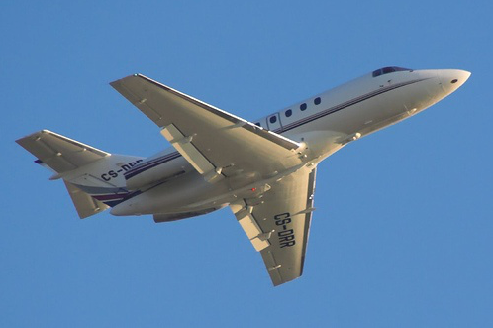
\includegraphics[scale=0.27]{bilder/flugzeug}}
\subfigure[Superpixelsegmentierung]{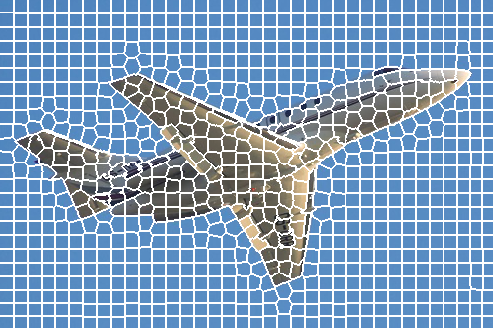
\includegraphics[scale=0.27]{bilder/flugzeug_slic}}
\subfigure[Graphrepräsentation]{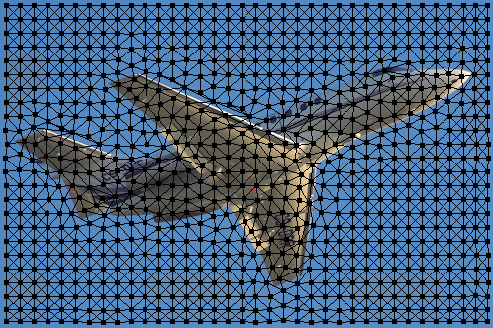
\includegraphics[scale=0.27]{bilder/flugzeug_slic_graph}}
\caption[Graphgenerierung aus einer Superpixelrepräsentation]{Illustration des Prozesses zur Graphgenerierung anhand einer Superpixelrepräsentation eines Bildes.
Ein Bild (a) wird dafür zuerst in eine Menge von Superpixeln segmentiert (b).
Die absoluten Zentren der Superpixel bilden die Knotenpunkte des Graphen.
Benachbarte Superpixel werden über eine Kante miteinander verbunden (c).}
\label{fig:superpixel_graph}
\end{figure}

Abbildung~\ref{fig:superpixel_graph} illustriert den beschriebenen Prozess der Graphgenerierung anhand einer Superpixelrepräsentation eines Bildes.

Zusätzlich zu der Positionsfunktion $p$ auf den Superpixelknoten kann der Graph \gls{G} um eine \emph{Massefunktion} $\gls{m} \colon \gls{V} \to \gls{N}$ mit $\gls{m}\left(\gls{v}_n\right) \coloneqq \left|S_n\right|$ zu $\gls{G} = \left(\gls{V}, \gls{E}, \gls{p}, \gls{m}\right)$ erweitert werden, die die Masse \bzw{} den Flächeninhalt der einzelnen Superpixelregionen beschreibt.

\paragraph{Effiziente Adjazenzbestimmung}
\label{adjazenzbestimmung_superpixel}

Die Bestimmung einer Kantenrelation \gls{E} auf einer Superpixelrepräsentation kann aufgrund der pixelweisen Iteration auf der Segmentierungsmaske und dem sukzessiven Vergleich mit den jeweiligen Nachbarspixeln über ein $3 \times 3$ Fenster recht teuer werden.
Eine effizientere und zugleich elegantere Bestimmung einer Kantenrelation als ungewichtete Adjazenzmatrix kann über eine versetzte Überlagerung der Segmentierungsmasken gewonnen werden.
Sei dafür $\gls{Smaske} \in {\left\{1, \ldots N\right\}}^{H \times W}$ eine Segmentierungsmaske.
Dann wird für die vertikale Adjazenzbestimmung die oberste und unterste Reihe aus \gls{Smaske} abgeschnitten und in $\gls{Smaske}_{\uparrow}, \gls{Smaske}_{\downarrow} \in {\left\{1, \ldots N\right\}}^{H-1 \times W}$ gespeichert.
$\gls{Smaske}_{\uparrow}$ und $\gls{Smaske}_{\downarrow}$ werden anschließend paarweise auf Ungleichheit getestet und dessen boolsches Ergebnis in einer Binärmaske $\left(\gls{Smaske}_{\uparrow} \neq \gls{Smaske}_{\downarrow}\right)$ gespeichert.
Liegen dabei wahre, \dhe{} ungleiche Einträge vor, so ist eine vertikale Adjazenz zwischen zwei unterschiedlichen Regionen vorhanden.
Die Einträge $i,j \in \left\{1, \ldots N \right\}$ in $\gls{Smaske}_{\uparrow}$ und $\gls{Smaske}_{\downarrow}$ an den Koordinaten der wahren Einträge in der Binärmaske bilden folglich die Knotenindizes einer Kante $\left(\gls{v}_i, \gls{v}_j\right) \in \gls{E}$ benachbarter Regionen und werden in eine Adjazenzmatrix mit $\gls{A}_{ij}=1$ übertragen.
Analog wird für die horizontale Adjazenzbestimmung vorgegangen.
\begin{figure}[t]
\centering
\subfigure[]{
$\begin{aligned}
  \gls{Smaske} = \begin{bmatrix}
    1 & 1 & 2 & 3\\
    1 & 2 & 2 & 3\\
    1 & 1 & 4 & 4
  \end{bmatrix}
\end{aligned}$
\begin{tikzpicture}[overlay]
  \draw[thick] (-1.85, 0.39) -- (-1.35, 0.39);
  \draw[thick] (-1.85, -0.125) -- (-0.275, -0.125);
\end{tikzpicture}
}
\subfigure[]{
$\begin{aligned}
  \gls{Smaske}_{\uparrow} = & \begin{bmatrix}
      1 & 2 & 2 & 3\\
      1 & 1 & 4 & 4
    \end{bmatrix}\\
      \gls{Smaske}_{\downarrow} = & \begin{bmatrix}
      1 & 1 & 2 & 3\\
      1 & 2 & 2 & 3
    \end{bmatrix}\\
    \left(\gls{Smaske}_{\uparrow} \neq \gls{Smaske}_{\downarrow}\right) = & \begin{bmatrix}
      \times & \checkmark & \times & \times\\
      \times & \checkmark & \checkmark & \checkmark\\
    \end{bmatrix}
\end{aligned}$
}
\subfigure[]{
  $\begin{aligned}
    \left(2,1\right) \in \gls{E},\,\,\,\, & \left(1,2\right) \in \gls{E}\\
    \left(4,2\right) \in \gls{E},\,\,\,\, & \left(4,3\right) \in \gls{E}\\
    \left(\gls{A} \vee \gls{A}^{\top}\right) = & \begin{bmatrix}
    0 & 1 & 0 & 0\\
    1 & 0 & 0 & 1\\
    0 & 0 & 0 & 1\\
    0 & 1 & 1 & 0
  \end{bmatrix}
\end{aligned}$
}
  \caption[Effiziente Adjazenzbestimmung einer Segmentierungsmaske]{Adjazenzbestimmung einer Segmentierungsmaske $\gls{Smaske} \in {\left\{1,2,3,4\right\}}^{3 \times 4}$ mit eingezeichneten vertikalen Adjazenzen (a).
  Daraus lassen sich $\gls{Smaske}_{\uparrow}$, $\gls{Smaske}_{\downarrow}$ sowie $\gls{Smaske}_{\uparrow} \neq \gls{Smaske}_{\downarrow}$ bestimmen (b).
  Die Einträge in $\gls{Smaske}_{\uparrow}$ und $\gls{Smaske}_{\downarrow}$ an den Indizes der wahren Werte in $\gls{Smaske}_{\uparrow} \neq \gls{Smaske}_{\downarrow}$ bilden jeweils eine Kante im Graphen (c).}
\label{fig:adjazenz}
\end{figure}

Die Veroderung $\gls{A} \vee \gls{A}^{\top}$ liefert dann die resultierende ungerichtete, ungewichtete Adjazenzmatrix mit einer Konnektivität von $4$ (\vgl{}~\cite{stackoverflow}).
Abbildung~\ref{fig:adjazenz} illustriert das Verfahren anhand eines einfachen Beispiels.

\paragraph{Globale und lokale Normierung}
\label{globale_lokale_normierung}

Eine Menge generierter Graphen aus den Superpixelrepräsentationen einer Bildermenge können sich zu Teilen extrem unterscheiden, \bspw{} durch variierende Auflösungen der Bilder.
So besitzt ein Graph möglicherweise nur sehr \enquote{kurze} Kanten, wohingegen ein anderer im Vergleich dazu ausschließlich aus \enquote{längeren} Kanten besteht.
Das kann bei der Transformation solcher Graphen in die Adjazenzmatrixrepräsentation $\gls{Adist} \in {\left[0, 1\right]}^{N \times N}$ aufgrund der Wahl des Parameters $\gls{sigma} \in \gls{R}$ zu Problemen führen.
Eine statische Wahl des Parameters \gls{sigma} führt dann \ggf{} zu Einträgen in \gls{Adist}, die stets sehr nahe bei Eins \bzw{} Null liegen.
Eine Normierung der Kantenlängen erscheint daher für die Transformation nach \gls{Adist} sinnvoll.
Eine \emph{Normierung} eines Graphen \gls{G} sieht dafür bei der Transformation nach \gls{Adist} eine Skalierung von ${\left\|\gls{p}\left(\gls{v}_i\right) - \gls{p}\left(\gls{v}_j\right)\right\|}_2^2 \in \gls{R}$ in das Intervall $\left[0, 1\right]$ vor.
Eine \emph{globale Normierung} von \gls{G} skaliert dabei ${\left\|\gls{p}\left(\gls{v}_i\right) - \gls{p}\left(\gls{v}_j\right)\right\|}_2^2$ über die maximale Kantenlänge ${\left\|\cdot\right\|}_2^2$ aller Kanten des Graphen, wohingegen die \emph{lokale Normierung} lediglich eine Skalierung über die maximale Kantenlänge der ausgehenden Kanten von $\gls{v}_i \in \gls{V}$ vorsieht.
Durch die lokale Normierung ist die Adjazenzmatrix \gls{Adist} insbesondere gerichtet.
Ein üblicher Trick, um dem entgegenzuwirken, ist die Aufsummierung von \gls{Adist} mit ihrer transponierten Matrix $\gls{Adist}^{\top}$ und der anschließenden Halbierung ihrer Werte, \dhe{} $\frac{1}{2}\left(\gls{Adist} + \gls{Adist}^{\top}\right)$~\cite{Reuter}.

Es ist anzumerken, dass der normierte Graph, repräsentiert als \gls{Adist}, neben der bereits vorhandenen Translationsinvarianz insbesondere skalierungsinvariant ist.
Im weiteren Verlauf dieser Arbeit wird der Prozess der Normierung eines Graphen implizit angenommen.
